\section{R-FCN}
% motivation for creating this theme
\begin{frame}{R-FCN}{Architecture}
\begin{columns}
    \column{0.5\textwidth}
        \begin{block}{Advances in FCNs}
        \begin{itemize}
            \item Convolutional model for computation of feature maps
            \begin{itemize}
                \item AlexNet, VGG, ResNets, etc
            \end{itemize}
            \item RPN for region proposals
            \item Position-sensitive score maps
        \end{itemize}
    \end{block}
    \column{0.5\textwidth}
        \begin{figure}
            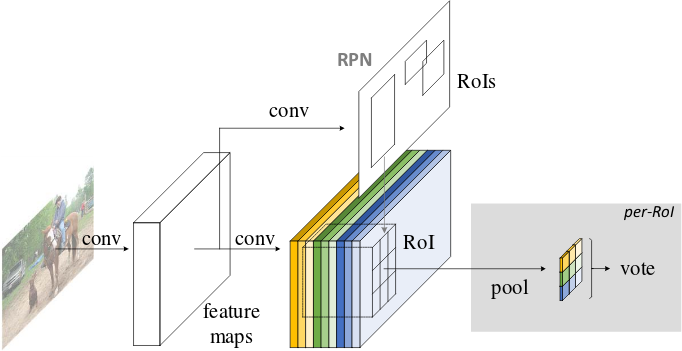
\includegraphics[width=1.0 \textwidth]{figs/rfcnarchi.png}
        \end{figure}
    \end{columns}
\end{frame}

\begin{frame}{R-FCN}{Region Proposal Network}
\begin{columns}
    \column{0.5\textwidth}
        \begin{block}{Finding potential objects}
        \begin{itemize}
            \item Class-agnostic region proposals
            \item Found using pre-defined anchors
            \item Regressed to fit potential bounding boxes
        \end{itemize}
    \end{block}
    \column{0.5\textwidth}
        \begin{figure}
            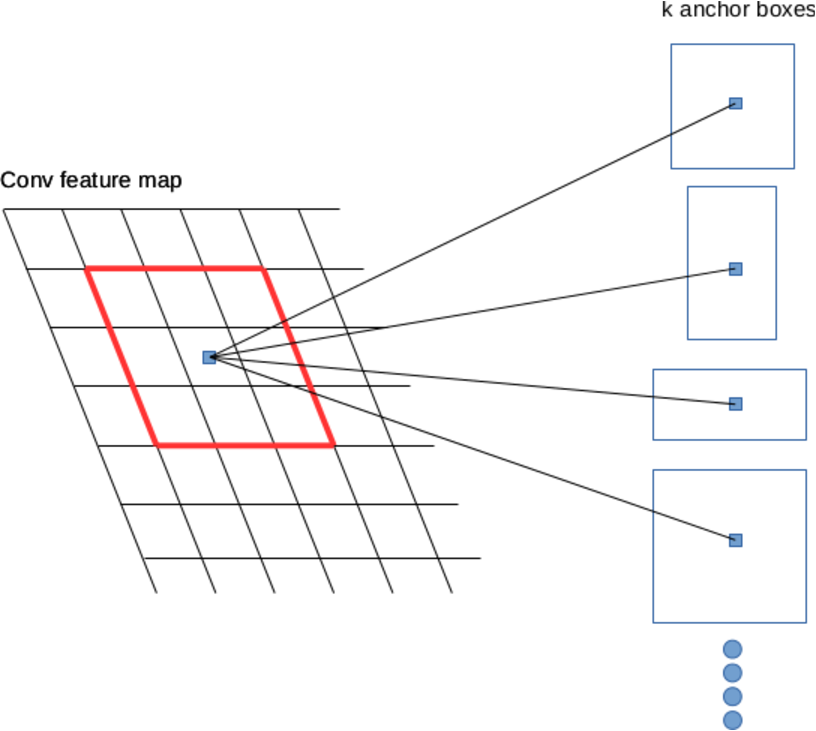
\includegraphics[width=1.0 \textwidth]{figs/rpn.pdf}
        \end{figure}
    \end{columns}
\end{frame}

\begin{frame}{R-FCN}{Position-Sensitive Score Maps}
\begin{columns}
    \column{0.3\textwidth}
        \begin{block}{Translation-invariant classification}
        \begin{itemize}
            \item Relative position score maps
            \item RPN proposal pooling
            \item Decision vote
        \end{itemize}
    \end{block}
    \column{0.7\textwidth}
        \begin{figure}
            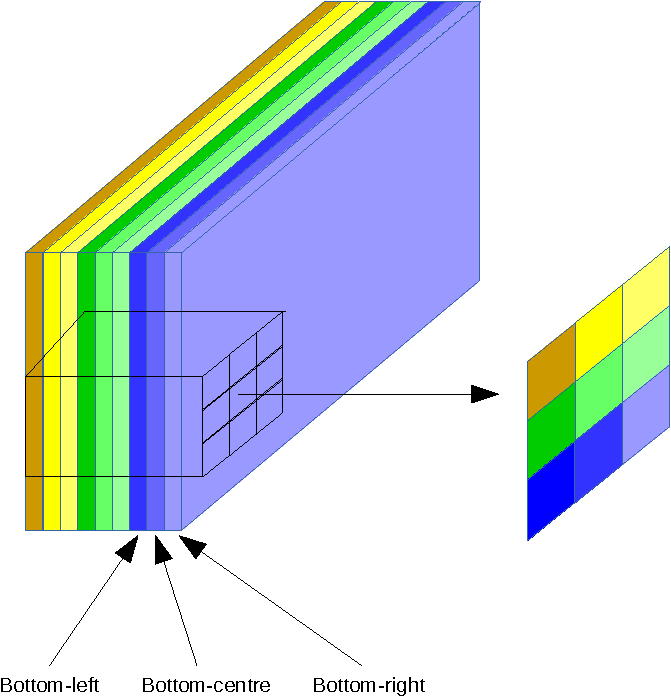
\includegraphics[width=0.3 \textwidth]{figs/scoremaps.pdf}
        \end{figure}
        \begin{figure}
            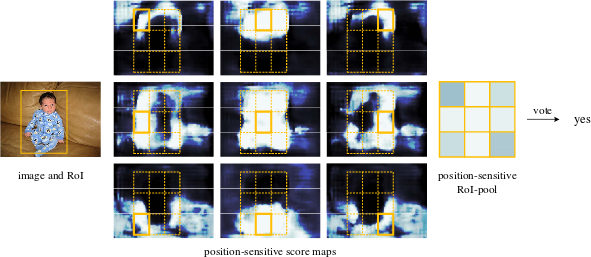
\includegraphics[width=0.7 \textwidth]{figs/rfcnpooling.png}
        \end{figure}
    \end{columns}
\end{frame}

\begin{frame}{Residual Networks}{Backbone Model}
\begin{columns}
    \column{0.5\textwidth}
        \begin{block}{Deep Representations}
        \begin{itemize}
            \item Intuition that deeper means better networks
            \begin{itemize}
                \item Not the case with VGG-inspired
            \end{itemize}
            \item Presented residual mappings in CNNs
        \end{itemize}
    \end{block}
    \column{0.5\textwidth}
        \begin{figure}
            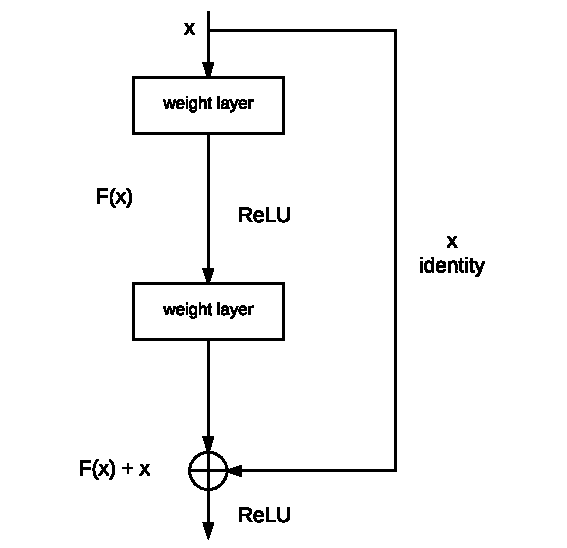
\includegraphics[width=1.0 \textwidth]{figs/resblock.pdf}
        \end{figure}
    \end{columns}
\end{frame}

\begin{frame}{Residual Networks}{Backbone Model}
\begin{columns}
    \column{0.5\textwidth}
        \begin{block}{State-of-the-art Classification}
        \begin{itemize}
            \item Residual block
            \item 50, 101, 152 common depths
            \item Newer inspirations
            \begin{itemize}
                \item 1000 layers
                \item etc
            \end{itemize}
        \end{itemize}
    \end{block}
    \column{0.5\textwidth}
        \begin{figure}
            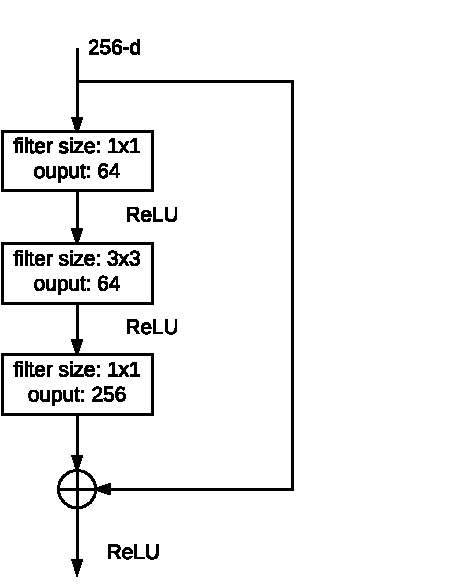
\includegraphics[width=0.8 \textwidth]{figs/newresblock.pdf}
        \end{figure}
    \end{columns}
\end{frame}